\documentclass{beamer}
\usepackage[utf8]{inputenc}
\usepackage{url}
\usetheme{Hokie}
\logo{
\includegraphics[height=0.5cm]{VTLogo.png}}
\setbeamertemplate*{logo}


\title{CMDA 4864 Beamer \& Markdown}
\author{CMDA 4864 GTA Team }
\subtitle{A Presentation on Presentations}
\date{November 2018}

\begin{document}

\frame{\titlepage}

%%%%%%%%%%%%%%%%%%%%%%%%%%%%%%%%%%%%%%%%%%%%%%%%%%%%%%%%%%
% Beamer Slides
%%%%%%%%%%%%%%%%%%%%%%%%%%%%%%%%%%%%%%%%%%%%%%%%%%%%%%%%%%
\begin{frame}{Beamer Basics}
\begin{itemize}
\item Beamer is a class of documents in \LaTeX that can create pdf slide presentations.
\item If you can write documents in \LaTeX, then its a simple extension to create Beamer presentations.
\item Advantages:
\begin{itemize}
\item You can easily import code from Tech Memos into your Final Presentation. 
\item Mathematical expressions typeset very well. 
\item Overleaf support.
\end{itemize}
\end{itemize} 
\end{frame}


\begin{frame}{Frames and Slides}
\begin{itemize}
\item Beamer presentations are made up of \alert{frames}.
\item Frames can be thought as a combination of slides/overlays.
\item One has easier control over how things are revealed in a frame, to emphasize particular text.
\end{itemize}
\end{frame}


\begin{frame}{Pause}
\begin{itemize}
\item Perhaps I start with the first point.
\item\pause Go on to my second,
\item and third point.
\end{itemize}
\pause
\begin{block}{Blocked Section Example}
Then end with a \alert{major takeway}.
\end{block}
\end{frame}


\begin{frame}{Two Column Example}
\begin{columns}
\begin{column}{0.5\textwidth}

\begin{itemize}
    \item Similar to Google Slides \& PowerPoint, one can split frames into columns.
    \item Perhaps place text on one side, and an image on the other side.
\end{itemize}

\end{column}
\begin{column}{0.5\textwidth}

    \begin{center}
     
\includegraphics[width=0.5\textwidth]{VTLogo.png}   
     \end{center}

\end{column}
\end{columns}
\end{frame}

\frame
{
	\frametitle{Example Table}
	
	\begin{table}
	\centering
	\begin{tabular}{|c|c|c|} \hline \hline
	Restrained     & Swivel         & Telemetry      \\ \hline \hline
	$\sim$ 400bpm  & $\sim$ 380bpm  & $\sim$ 310 bpm \\
	$\sim$ 140mmHg & $\sim$ 120mmHg & $\sim$ 100mmHg \\ \hline \hline
	\end{tabular}
	\caption{Heart beat and blood pressure using different monitoring methods}
	\label{tbl:kramer}
	\end{table}
}

\begin{frame}{Other Resources}
\begin{itemize}
    \item There are plenty of resources!
    \item \textbf{Beamer Documentation on CTAN} \\ \url{https://ctan.org/tex-archive/macros/latex/contrib/beamer/doc/}
    \item \textbf{In depth presentation} \\
    \url{https://www.uncg.edu/cmp/reu/presentations/Charles\%20Batts\%20-\%20Beamer\%20Tutorial.pdf}
    \item \textbf{Overleaf Demos} \\
    \url{https://www.overleaf.com/learn/latex/Beamer_Presentations:_A_Tutorial_for_Beginners_(Part_1)\%E2\%80\%94Getting_Started}
\end{itemize}
\end{frame}

%%%%%%%%%%%%%%%%%%%%%%%%%%%%%%%%%%%%%%%%%%%%%%%%%%%%%%%%%%
% R Markdown Slides
%%%%%%%%%%%%%%%%%%%%%%%%%%%%%%%%%%%%%%%%%%%%%%%%%%%%%%%%%%
% \begin{frame}{Introduction to Markdown}
Markdown is a text-to-HTML conversion tool for web writers. 
    
\end{frame}

\begin{frame}{Presentations using R markdown}

\begin{columns}
\begin{column}{0.45\textwidth}
R Markdown offers 3 types of presentations.
\begin{itemize}
    \item iosslides
    \item slidy
    \item beamer
\end{itemize}
\end{column}

\begin{column}{0.55\textwidth}
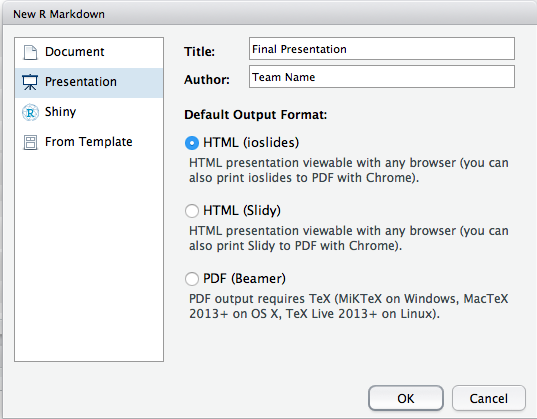
\includegraphics[width=2.5in]{RMarkdown/2.png}
\end{column}
\end{columns}

In R Studio:\\
\vspace{6pt}

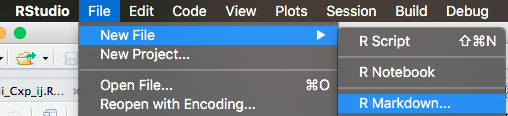
\includegraphics[width=2.5in]{RMarkdown/1.png}
\end{frame}

\begin{frame}{Preamble}
\begin{itemize}
\item For Beamer:\\
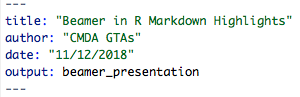
\includegraphics[width=3in]{RMarkdown/pre1.png}
\item For Iosslides:\\
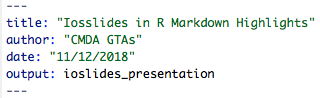
\includegraphics[width=3in]{RMarkdown/pre2.png}
\end{itemize}
\end{frame}

\begin{frame}{Render the Presentation}
\begin{itemize}
    \item To create a presentation, click \textbf{Knit}: 
\includegraphics[width=1in]{RMarkdown/4.png}
    \item Knit automatically renders in the designated output type.
    \item Change the output type by clicking the down arrow:\\
\centering 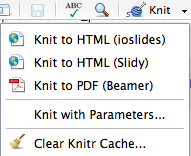
\includegraphics[width=2in]{RMarkdown/3.png}
\end{itemize}
\end{frame}

\begin{frame}{Markdown Basics}
\begin{table} \centering
    \begin{tabular}{r|l} \hline
    \textbf{Task} & \textbf{Command} \\ \hline
         New Slide & \#\#\\
         Bullets & $-$ or $*$ \\
         Italicize & $*$Example Text$*$ \\
         Bold & $**$Example Text$**$ \\
         Comment & $<!--$ Example Text $-->$\\ 
         \LaTeX & Use \$ or \$\$ \\ \hline
    \end{tabular}
\end{table}

For more information:
\begin{itemize}
    \item \url{https://rmarkdown.rstudio.com/lesson-11.html}
    % \item \href{https://www.rstudio.com/wp-content/uploads/2015/02/rmarkdown-cheatsheet.pdf}{R Markdown Cheatsheet}
\end{itemize}

\end{frame}

%%%%%%%%%%%%%%%%%%%%%%%%%%%%%%%%%%%%%%%%%%%%%%%%%%%%%%%%%%
% Presentations in Python Slides
%%%%%%%%%%%%%%%%%%%%%%%%%%%%%%%%%%%%%%%%%%%%%%%%%%%%%%%%%%

\begin{frame}{Other Language Engines}

Many other languages are also supported in R markdown, e.g., Python, Julia, C++, and SQL.
\vspace{5mm}

For more information:
\begin{itemize}
    \item \url{https://bookdown.org/yihui/rmarkdown/language-engines.html}
    \item \url{https://blog.rstudio.com/2018/03/26/reticulate-r-interface-to-python/}
\end{itemize}

    
\end{frame}


\begin{frame}{R Markdown Presentation Demos}
    
\begin{columns}
\begin{column}{0.38\textwidth}
Moving on to demo files:
\begin{itemize}
\item \url{Demo_Beamer.Rmd}
\item \url{Demo_Iosslides.Rmd}
\end{itemize}
\vspace{0.5in}

\emph{Note: To compile these files, need to have python.png and path to file updated.}
\end{column}

\begin{column}{0.6\textwidth}
\underline{Demo Outline:}
\begin{itemize}
    \item Setup
    \item Bulleted Lists
    \item R Example (Code and Output)
    \item Table in Markdown
    \item Table using Kable Function
    \item Plots
    \item Inserting Images
    \item Python Example (Code and Output)
\end{itemize}
\end{column}
\end{columns}
\end{frame}

\end{document}
